%%%%%%%%%%%%%%%%%%%%%%%%%%%%%%%%%%%%%%%%%
% Wenneker Article
% LaTeX Template
% Version 2.0 (28/2/17)
%
% This template was downloaded from:
% http://www.LaTeXTemplates.com
%
% Authors:
% Vel (vel@LaTeXTemplates.com)
% Frits Wenneker
%
% License:
% CC BY-NC-SA 3.0 (http://creativecommons.org/licenses/by-nc-sa/3.0/)
%
%%%%%%%%%%%%%%%%%%%%%%%%%%%%%%%%%%%%%%%%%

%----------------------------------------------------------------------------------------
%	PACKAGES AND OTHER DOCUMENT CONFIGURATIONS
%----------------------------------------------------------------------------------------

\documentclass[10pt, a4paper, twocolumn]{article} % 10pt font size (11 and 12 also possible), A4 paper (letterpaper for US letter) and two column layout (remove for one column)



%%%%%%%%%%%%%%%%%%%%%%%%%%%%%%%%%%%%%%%%%
% Wenneker Article
% Structure Specification File
% Version 1.0 (28/2/17)
%
% This file originates from:
% http://www.LaTeXTemplates.com
%
% Authors:
% Frits Wenneker
% Vel (vel@LaTeXTemplates.com)
%
% License:
% CC BY-NC-SA 3.0 (http://creativecommons.org/licenses/by-nc-sa/3.0/)
%
%%%%%%%%%%%%%%%%%%%%%%%%%%%%%%%%%%%%%%%%%

%----------------------------------------------------------------------------------------
%	PACKAGES AND OTHER DOCUMENT CONFIGURATIONS
%----------------------------------------------------------------------------------------

\usepackage[english]{babel} % English language hyphenation

\usepackage{microtype} % Better typography

\usepackage{amsmath,amsfonts,amsthm} % Math packages for equations

\usepackage[svgnames]{xcolor} % Enabling colors by their 'svgnames'

\usepackage[hang, small, labelfont=bf, up, textfont=it]{caption} % Custom captions under/above tables and figures

\usepackage{booktabs} % Horizontal rules in tables

\usepackage{lastpage} % Used to determine the number of pages in the document (for "Page X of Total")

\usepackage{graphicx} % Required for adding images

\usepackage{enumitem} % Required for customising lists
\setlist{noitemsep} % Remove spacing between bullet/numbered list elements

\usepackage{sectsty} % Enables custom section titles
\allsectionsfont{\usefont{OT1}{phv}{b}{n}} % Change the font of all section commands (Helvetica)

%----------------------------------------------------------------------------------------
%	MARGINS AND SPACING
%----------------------------------------------------------------------------------------

\usepackage{geometry} % Required for adjusting page dimensions

\geometry{
	top=1cm, % Top margin
	bottom=1.5cm, % Bottom margin
	left=2cm, % Left margin
	right=2cm, % Right margin
	includehead, % Include space for a header
	includefoot, % Include space for a footer
	%showframe, % Uncomment to show how the type block is set on the page
}

\setlength{\columnsep}{7mm} % Column separation width

%----------------------------------------------------------------------------------------
%	FONTS
%----------------------------------------------------------------------------------------

\usepackage[T1]{fontenc} % Output font encoding for international characters
\usepackage[utf8]{inputenc} % Required for inputting international characters

\usepackage{XCharter} % Use the XCharter font

%----------------------------------------------------------------------------------------
%	COLORS
%----------------------------------------------------------------------------------------

\definecolor{primary}{RGB}{126, 160, 183}
\definecolor{secondary}{RGB}{169, 206, 244}


%----------------------------------------------------------------------------------------
%	HEADERS AND FOOTERS
%----------------------------------------------------------------------------------------

\usepackage{fancyhdr} % Needed to define custom headers/footers
\pagestyle{fancy} % Enables the custom headers/footers

\renewcommand{\headrulewidth}{0.0pt} % No header rule
\renewcommand{\footrulewidth}{0.4pt} % Thin footer rule

\renewcommand{\sectionmark}[1]{\markboth{#1}{}} % Removes the section number from the header when \leftmark is used

%\nouppercase\leftmark % Add this to one of the lines below if you want a section title in the header/footer

% Headers
\lhead{} % Left header
\chead{\textit{\thetitle}} % Center header - currently printing the article title
\rhead{} % Right header

% Footers
\lfoot{} % Left footer
\cfoot{} % Center footer
\rfoot{\footnotesize Page \thepage\ of \pageref{LastPage}} % Right footer, "Page 1 of 2"

\fancypagestyle{firstpage}{ % Page style for the first page with the title
	\fancyhf{}
	\renewcommand{\footrulewidth}{0pt} % Suppress footer rule
}

%----------------------------------------------------------------------------------------
%	TITLE SECTION
%----------------------------------------------------------------------------------------

\newcommand{\authorstyle}[1]{{\large\usefont{OT1}{phv}{b}{n}\color{primary}#1}} % Authors style (Helvetica)

\newcommand{\keywords}[1]{Keywords: {\footnotesize\usefont{OT1}{phv}{m}{sl}\color{Black}#1}\vspace{5pt}} % Institutions style (Helvetica)

\usepackage{titling} % Allows custom title configuration

\newcommand{\HorRule}{\color{secondary}\rule{\linewidth}{1pt}} % Defines the gold horizontal rule around the title

\pretitle{
	\vspace{-30pt} % Move the entire title section up
	\HorRule\vspace{10pt} % Horizontal rule before the title
	\fontsize{32}{36}\usefont{OT1}{phv}{b}{n}\selectfont % Helvetica
	\color{primary} % Text colour for the title and author(s)
}

\posttitle{\par\vskip 15pt} % Whitespace under the title

\preauthor{} % Anything that will appear before \author is printed

\postauthor{ % Anything that will appear after \author is printed
	\vspace{10pt} % Space before the rule
	\par\HorRule % Horizontal rule after the title
	\vspace{20pt} % Space after the title section
}

%----------------------------------------------------------------------------------------
%	ABSTRACT
%----------------------------------------------------------------------------------------

\usepackage{lettrine} % Package to accentuate the first letter of the text (lettrine)
\usepackage{fix-cm}	% Fixes the height of the lettrine

\newcommand{\initial}[1]{ % Defines the command and style for the lettrine
	\lettrine[lines=3,findent=4pt,nindent=0pt]{% Lettrine takes up 3 lines, the text to the right of it is indented 4pt and further indenting of lines 2+ is stopped
		\color{secondary}% Lettrine colour
		{#1}% The letter
	}{}%
}

\usepackage{xstring} % Required for string manipulation

\newcommand{\lettrineabstract}[1]{
	\StrLeft{#1}{1}[\firstletter] % Capture the first letter of the abstract for the lettrine
	\initial{\firstletter}\textbf{\StrGobbleLeft{#1}{1}} % Print the abstract with the first letter as a lettrine and the rest in bold
}

%----------------------------------------------------------------------------------------
%	BIBLIOGRAPHY
%----------------------------------------------------------------------------------------

\usepackage[backend=bibtex]{biblatex} % Use the bibtex backend with the authoryear citation style (which resembles APA)

\addbibresource{example.bib} % The filename of the bibliography

\usepackage[autostyle=true]{csquotes} % Required to generate language-dependent quotes in the bibliography
 % Specifies the document structure and loads requires packages

%----------------------------------------------------------------------------------------
%	ARTICLE INFORMATION
%----------------------------------------------------------------------------------------

\title{Limitations of AI: the case against singularity} % The article title

\author{
	\authorstyle{V\'ictor Santiago Gonz\'alez} % Authors
	\newline\newline % Space before institutions
	\keywords{Artificial Intelligence, Singularity, Manifold Hypothesis, 
	Machine Learning, Neural networks, Limitations}\\ % Institution 1
}

% Example of a one line author/institution relationship
%\author{\newauthor{John Marston} \newinstitution{Universidad Nacional Autónoma de México, Mexico City, Mexico}}

\date{} % Add a date here if you would like one to appear underneath the title block, use \today for the current date, leave empty for no date


%----------------------------------------------------------------------------------------
%	ABSTRACT
%----------------------------------------------------------------------------------------

\postauthor{

	\begin{center}
		\textsc{\textbf{Abstract}}
	\end{center}
	
	Lorem ipsum dolor sit amet, consectetur adipiscing elit. Fusce maximus nisi ligula. Morbi laoreet ex ligula, vitae lobortis purus mattis vel. Vestibulum ante ipsum primis in faucibus orci luctus et ultrices posuere cubilia Curae; Donec ac metus ut turpis mollis placerat et nec enim. Duis tristique nibh maximus faucibus facilisis. Praesent in consequat leo. Maecenas condimentum ex rhoncus, elementum diam vel, malesuada ante.

	\par\vspace{10pt}\HorRule
}

%----------------------------------------------------------------------------------------

\begin{document}

\maketitle % Print the title

\thispagestyle{firstpage} % Apply the page style

%-------------------------------------------------------------------------------
%	ARTICLE CONTENTS
%-------------------------------------------------------------------------------

	%-------------------------------------------------------------------------------
	%	SINGULARITY
	%-------------------------------------------------------------------------------

	\section{The singularity about to come}

	The \textit{singularity} is a term first coined by Vernon Vinge and popularized, 
later on, by Ray Kurzweil in a series of books published by early 2000's.
\cite{age, singularity} 

It refers to a point in technologial progress (particularly in the field of 
Artificial Intelligence) where \textbf{machine's capabilities will overcome all human 
intelligence combined.}

Vinge's article hesitates to asses singularity's feasibility (He isn't 100\% sure 
but "If it can happen, It will", he concedes), Kurzweil stance is significatively 
more bold: \textit{he actually made predictions.}\footnote{
	It is relevant noticing that Mr. Kurzweil, Google's director of engineering, 
	is a reputated futurist. Thus, we can see the predictions listed above as a 
	curated summary on Artificial Intelligence's \textit{state of the buzz}
}

Regarding artificial intelligence, the steps that will pave the road to the 
singularity are\cite{interview}: 

\begin{itemize}
	\item [\textbf{\textcolor{secondary}{2009}}] Speech-to-speech automated 
		translation will be available in cell phones.

	\item [\textbf{\textcolor{secondary}{2017}}] Computers will be ubiquitous, 
		smaller, integrated in our clothes and some of them sel-organized.

	\item [\textbf{\textcolor{secondary}{2017}}] Full inmersive virtual reality 
		will be available.
	
	\item [\textbf{\textcolor{secondary}{2018}}] 10TB of memory storage (roughly 
		the human brain capacity) will cost less than \$1000.

	\item [\textbf{\textcolor{secondary}{2020}}] A computer is expected to pass 
		Türing's test. 

	\item [\textbf{\textcolor{secondary}{2023}}] $10^16$ calculations per second 
		will be possible in a cheap machine.

	\item [\textbf{\textcolor{secondary}{2029}}] Computers will have achieved 
		human-level intelligence.

	\item [\textbf{\textcolor{secondary}{2025}}] Military-grade UAV's will be 
		100\% autonomous.

	\item [\textbf{\textcolor{secondary}{2045}}] \textbf{Singularity}. Artificial 
		Intelligences will became the smartest and most skilled creatures in earth.

\end{itemize}

Kurzweil's confidence is built on top of \textit{"The law of accelerated returns"}, \cite{law}, 
which states that: 

\textcolor{gray}{
	\textit {
		\Large {
			"Rate of progress of an evolutionary process increases exponentially 
			[and] technology is such another evolutionary progress"
		}
	}
}

Reallity seems to follow Kurzweil's predictions: it is possible to buy a 10TB 
Seagate Barracuda for $\sim400$\euro{}, Virtual (or augmented) reality systems 
have become popular in the last few years, Machine's translation has seen 
spectacular\footnote{
	It's not only Google Translate new arquitecture, it worth to mention Waverly Labs's 
	earphones\cite{pilot}, a new gadget that promises live and wearable machine translation.
} advances... 

And inspite of, in practice, every exponential growth is exponential until is not,
Microprocesors industry have conformed Moore's Law (an equivalent formulation of 
the same principle) for decades.

But most of machine learning's whispering are built on top of modern neural network
capabilities. After the publication of backpropagation \cite{back} algorithm, and the rise 
of cloud computing, neural network applications have grown rapidly. Nowadays, 
finding impressive examples of neural networks adopting nearly-human behaviours 
is susrprisingly easy: 

\begin{itemize}
	\item They can \textit{dream}.\cite{dream}
	\item They describe pictures, bettern than most human journalist do.\cite{caption}
	\item They can code a website by their own.\cite{code}
	\item They are playing video games.\cite{snake}
\end{itemize}

The temptation to attribute human behaviour to AI systems is stronger today than 
it ever was. Therefore it looks that we should agree Mr Kurzweil: the singularity 
is near. 

Is it?

	%-------------------------------------------------------------------------------
	%	LIMITATIONS
	%-------------------------------------------------------------------------------

	\section{Something is rotten in \textit{the state of the art}}

	The problem of antrhopomorphizing machine learning applications is that, often, 
those statements come from marketing departments or reporters who've ever trained 
a model. They haven't realized (or deliberately omit) an obvious flaw that all 
the algorithms and techniques share in practice: \textbf{they don't train, they 
are trained by humans.}

Actually, there is an incredibly ammount of human work in every machine learning 
project that comes from human labour, including: 

\begin{itemize}
	\item \textbf{Data preparation:} every model has his own requirements about 
		data format. 
	\item \textbf{Data cleansing:} most algorithms assume that their training 
		phase will be conducted over a perfectly curated data set: \textit{
		zip codes that actually refer geographical information, missing data 
		to be imputed...}
	\item \textbf{Context awareness:} That's specially important in the case 
		of neural networks. Way before running the first epoch, the researcher 
		or data scientist, must figure out how to express problem's logic in a 
		language that the network can deal with. Sometimes this represent a 
		straightforward requirement, sometimes is nearly impossible. 
	\item \textbf{Disambiguation, cultural biases:} Machine learning inherits \cite{gorilla}
		all sort of biases included in the training dataset. It's human responsability 
		to prune them.  
\end{itemize}

Event thought their inherent difficulty and prevalence, the aforementioned arguments 
could be considered \textit{low-level} tasks in the context of artificial 
intelligence. Not a real concern for the \textit{singularity} concept.

Specially if we assume Kurzweil's full thesis, i.e., that the singularity will 
reach by a mixed human and artificial intelligence. What he called \textit{human 
2.0} would be a human body empowered with the benefits of the kind of \textit{
learning} we associate with current machine learning or deep learning systems.

On the one hand, this scenario would overcome all the problems mentioned until now: 
the human brain will still be there to manage them. But, in the other hand, all what w
we did adopting the \textit{human 2.0} argument is changing the perspective. Now 
the questions look different.

\textcolor{primary}{
\textbf{How reliable this brand new learning is?}
}

Sadly, in practice, even slightly departures from the nature of training data could
turn the finest tuned models into completely absurd predictors.

Recent research on "adversarial examples"\cite{adversarial} has shown how adding 
noise (inperceptible to human eye) to well classified images can substantially modify 
the output.

\begin{figure}[h!]
	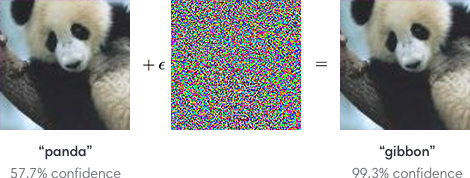
\includegraphics[width=\linewidth]{images/panda.png} % Figure image
	\caption{Adding noise ruin the predictions} % Figure caption
	\label{bear} % Label for referencing with \ref{bear}
\end{figure}

The system starts, suddenly, saying that panda bears are gibbons; \cite{panda} or refuses to 
recognize image's contents depending on the process followed to capture them.

\textbf{Deep learners, learn. But they don't understand.}

\textcolor{primary}{
\textbf{You want me to become a cyborg, right? Does it worth? Will it add 
something fundamentally valuable to my current intelectual toolbox?}
}

Regarding this question (which, basically, inquires on what are the theoretical 
limitations of machine learning) we should consider John Lauchbury's \textit{
"manifold hypothesis"} \cite{darpa} 

In short, this hypothesis states a generalization to a high-dimensional space 
of the well-known linear separability problem. Where a simple perceptron isn't 
able to \textit{learn} a non-linearly separable group of clusters in a given 
dataset; the extension to multidimensional spaces considers that clusters adopt 
the form of manifolds and entangled manifolds that cannot be separated produce 
datasets that cannot be learned.

This geometric stance links the problem of deciding when culstering (or 
"classification" or "learning") can be performed over a general dataset with 
the mathematical field of topological manifolds, particularly with the question 
of entangled manifolds separability.\cite{topology}

Both questions lack from a general answer. But the adoption of this \textit{
geometrical} view fills one important gap in some machine learning (deep or not) 
setups: the explainability of the models after training.

Lookgin through the topology glass, neural networks have only one job: to perform 
continuous transformations between spaces. 

	\begin{figure}[h!]
\begin{center}
		
\includegraphics[height=5cm]{images/baby.jpg} % Figure image
		\caption{Artificially generated caption: toothbrush $=$ bat} % Figure caption
		\label{baby} % Label for referencing with \ref{bear}
\end{center}
	\end{figure}

And humans are overwhelmingly good at it. That's why we'd never confuse a bat 
with a toothbrush.  


	%-------------------------------------------------------------------------------
	%	LIMITATIONS
	%-------------------------------------------------------------------------------

	\section{Good old intelligence}

	At this point, our assesment of machine intelligence is quite negative: they 
aren't capable to perform the most basic tasks they need to start working, they 
can't contextualize their scope. They aren't understanding the problems they 
claimed to had learnt. And they aren't using any magical reasoning, but basic 
geometric transformations.

Still, someone could argue (maybe Mr Kurzweil himself) that some systems are 
outperforming humans in some areas: Didn't Deep Blue win Kasparov? Didn't IBM's 
Watson win Jeopardy?

No, they didn't.

None of these machines decided by its own to train his skills in order to 
participate in the contest. Humans did.

And this is a big \textit{no}. Because, in my opinion, what truly defines 
intelligence is

\textcolor{gray}{
	\Large{
		the ability to come up with questions, not the ability to provide 
		answers.
	}
}

Chances are that the post-singularity world (if any) will be populated by 
millions of super-skilled machines quietly waiting for instructions. Doing nothing.

	%-------------------------------------------------------------------------------
	%	CONCLUSION
	%-------------------------------------------------------------------------------

	\section{Conclusions}

	Lorem ipsum dolor sit amet, consectetur adipiscing elit. Fusce maximus nisi ligula. Morbi laoreet ex ligula, vitae lobortis purus mattis vel. Vestibulum ante ipsum primis in faucibus orci luctus et ultrices posuere cubilia Curae; Donec ac metus ut turpis mollis placerat et nec enim. Duis tristique nibh maximus faucibus facilisis. Praesent in consequat leo. Maecenas condimentum ex rhoncus, elementum diam vel, malesuada ante. Fusce pulvinar, mauris pretium placerat venenatis, lectus ex tempus lacus, id suscipit libero lorem eu augue. Interdum et malesuada fames ac ante ipsum primis in faucibus.

Lorem ipsum dolor sit amet, consectetur adipiscing elit. Fusce maximus nisi ligula. Morbi laoreet ex ligula, vitae lobortis purus mattis vel. Vestibulum ante ipsum primis in faucibus orci luctus et ultrices posuere cubilia Curae; Donec ac metus ut turpis mollis placerat et nec enim. Duis tristique nibh maximus faucibus facilisis. Praesent in consequat leo. Maecenas condimentum ex rhoncus, elementum diam vel, malesuada ante. Fusce pulvinar, mauris pretium placerat venenatis, lectus ex tempus lacus, id suscipit libero lorem eu augue. Interdum et malesuada fames ac ante ipsum primis in faucibus.

Lorem ipsum dolor sit amet, consectetur adipiscing elit. Fusce maximus nisi ligula. Morbi laoreet ex ligula, vitae lobortis purus mattis vel. Vestibulum ante ipsum primis in faucibus orci luctus et ultrices posuere cubilia Curae; Donec ac metus ut turpis mollis placerat et nec enim. Duis tristique nibh maximus faucibus facilisis. Praesent in consequat leo. Maecenas condimentum ex rhoncus, elementum diam vel, malesuada ante. Fusce pulvinar, mauris pretium placerat venenatis, lectus ex tempus lacus, id suscipit libero lorem eu augue. Interdum et malesuada fames ac ante ipsum primis in faucibus.


%----------------------------------------------------------------------------------------
%	BIBLIOGRAPHY
%----------------------------------------------------------------------------------------

\printbibliography[title={References}] % Print the bibliography, section title in curly brackets

%----------------------------------------------------------------------------------------

\end{document}
